% !TEX root = ../tjumain.tex
\chapter{报告摘要}

随着时代的发展,网络技术日新月异,为了能够对网络技术的底层设计哲学有更深层的理解,我们参与并完成了本次关于 TCP 协议在应用层实现的实践任务。我们首先根据 RFC 793 文档设计了基于应用层的实现逻辑。然后使用C语言,在统一的 Ubuntu环境(见图\ref{fig:ubuntu})下进行了协议实体的代码实现。实现了包括\textbf{“连接管理”,“可靠数据传输”,“流量控制”,“连接关闭”和“拥塞控制”}等功能。并对吞吐率进行了验证,验证了协议实现的正确性。

\begin{figure}[!htbp]
  \centering
  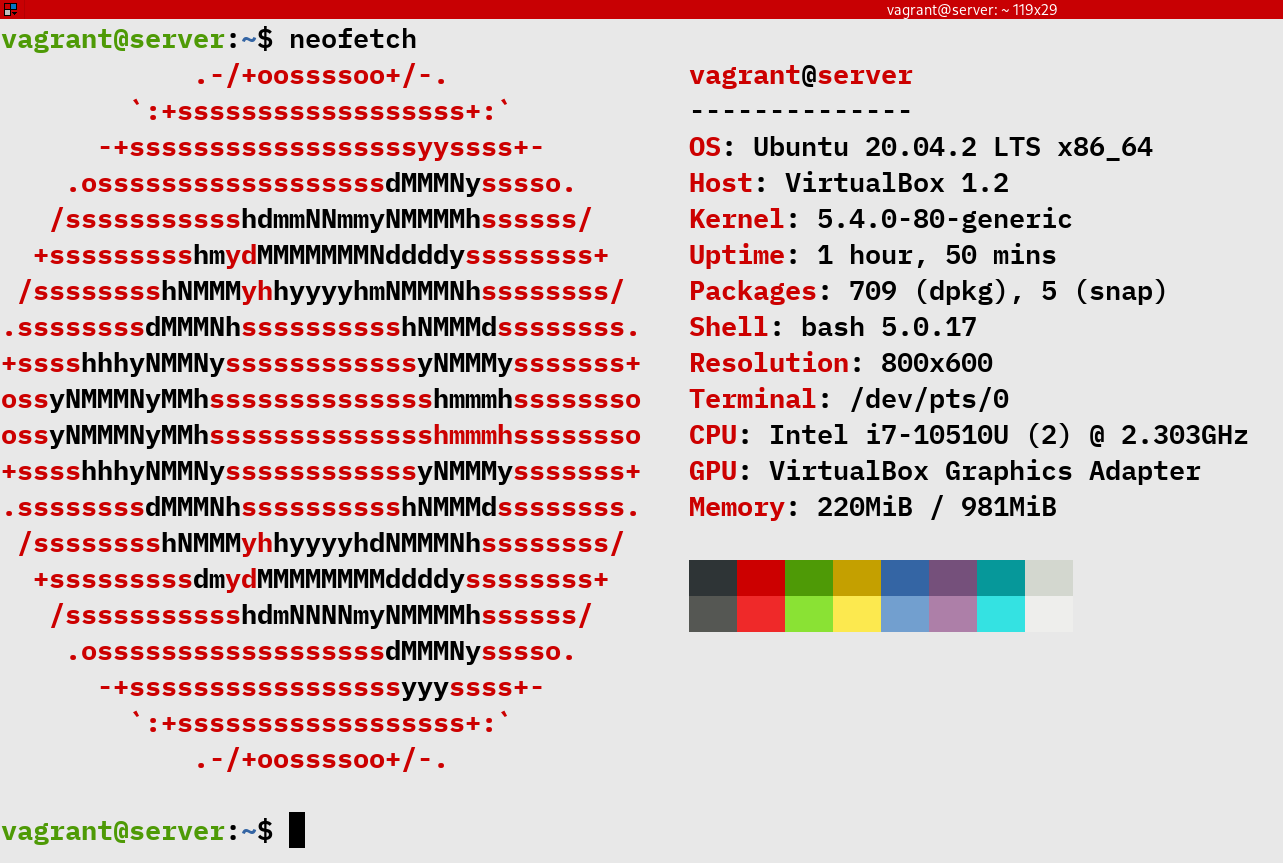
\includegraphics[width=1.0\textwidth]{_ubuntu.png}
  \label{fig:ubuntu}\caption{测试环境信息}
\end{figure}

协议设计分为六个部分,将在第三章进行重点介绍,设计的重点在于将RFC 793 文档的文字进行逻辑翻译。程序总共\textbf{三个线程},使用一个接收线程处理接收到的包裹、发送 ACK以及将内容递交给上层实体;使用一个发送线程从上层实体接收待发送的包,并进行可靠数据传输;最后一个应用层的用户端主线程。

我们\textbf{顺利通过了三次线上的测试以及拥塞控制和性能测试等额外测试}(拥塞控制并没有来得及提交报告,在本报告中统一进行阐述)。

